\maketitle

\begin{abstract}
	In response to the critical need for efficient wildfire detection, this study presents a novel approach leveraging machine learning techniques applied to images from ground cameras and drones. Traditional methods, predominantly relying on satellite imagery, often grapple with false positives and maintenance challenges. Our method aims to address these limitations by utilizing a more direct and responsive source of visual data. The significance of this research is underscored by California's substantial investment in wildfire management, with CalFire allocating \$3.3 billion annually for this purpose. The proposed system, therefore, has the potential to significantly reduce costs and enhance early detection capabilities, particularly in remote areas.
	We curated a comprehensive dataset of 843,862 images, categorized into fire and non-fire classes, from a 16GB image repository sourced from Kaggle. To optimize memory usage and enable efficient batch processing, images were resized to 200×200 pixels. Duplicate removal was achieved through image hashing, and data augmentation techniques expanded our dataset fivefold. This included modifications in zoom, brightness, color jittering, Gaussian noise, and horizontal flipping. All images were standardized to JPEG format.
	For model development, we employed an 80\%-20\% split for training and testing, and an 85\%-15\% split for training and validation. The study experimented with various neural networks, including ResNet, MobileNet, and AlexNet, over 10 epochs using SGD optimization with a momentum of 0.9 and a learning rate of 0.001. ResNet emerged as the most effective model, benefiting from deeper layers and skip connections. MobileNet, while efficient, lacked the complexity needed for pattern recognition, and AlexNet's simpler architecture led to lower performance.
	To enhance the robustness of our model against overfitting, we are considering the implementation of k-fold cross-validation. Additionally, we plan to integrate semantic segmentation for more precise fire localization. Future work will focus on augmenting the dataset with edge case images, particularly those with various light sources, to improve the model's resistance to false positives. This research not only contributes to the field of wildfire detection but also demonstrates the potential of machine learning in addressing environmental and public safety challenges.
\end{abstract}

\section{Introduction}

In the realm of wildfire management and prevention, the development of an advanced early fire detection system stands as a critical innovation. Traditional methods, primarily relying on satellite imagery, are increasingly proving inadequate due to their susceptibility to false positives and ongoing maintenance challenges. To address these limitations, our research introduces a novel approach utilizing Computer Vision (CV) technology, harnessing images from ground-based cameras and drones. This methodology marks a significant leap in accurately identifying the presence of fire, particularly in its nascent stages.

The urgency and importance of this development are underscored by the efforts of organizations such as CalFire. As the state agency responsible for fire protection and the stewardship of over 31 million acres of California's wildlands, CalFire's expenditure of \$3.3 billion for wildfire protection and suppression vividly illustrates the substantial financial and environmental stakes involved. ~\citep{calfire} This immense budget not only highlights the state's commitment to managing and responding to wildfires but also reflects the enormous economic impact of these natural disasters.

In this context, the potential of an early fire detection system cannot be overstated. By enabling quicker and more accurate detection of wildfires, especially in remote or hard-to-reach areas where traditional surveillance methods are limited, such a system could have a profound economic effect. The anticipated benefits include significant cost savings, potentially amounting to millions of dollars annually, and more importantly, the mitigation of extensive environmental and property damage. Our research aims to explore and validate the effectiveness of this CV-based system, positioning it as a pivotal tool in the ongoing battle against wildfires.


Detecting fires from a set of images

Building a computer vision model that can classify fire/no-fire from an image

We use ground-based imagery which is real-time and less expensive while generating high resolution images

Data augmentation allows our model to generalize better and improve our model’s ability to detect fires in various scenarios

Hyperparameter tuning allows us to find the optimal configuration for our model

Can easily be expanded by leveraging contextual information, such as weather data or land use information, to help distinguish between different types of fires

We used pre-trained deep learning models such as ResNet for feature extraction which can also be fine-tuned for better generalization via transfer learning

\section{Related Work}

Over-reliance on smoke detection: not all fires cause smoke, which can delay fire detection

Maintenance issues such as sensor calibration problems or battery failures
False positives that can be triggered by cooking smoke, steam, dust, or other airborne particles

Satellite imagery for wildfire detection is vulnerable to atmospheric conditions, low resolution, and lack of real-time monitoring

\subsection{How We Are Better}

Velit adipisicing ullamco dolor deserunt laboris. Veniam culpa ex reprehenderit adipisicing tempor amet reprehenderit amet pariatur adipisicing dolor fugiat occaecat enim. Cillum commodo sit voluptate est tempor esse elit exercitation. Et cupidatat id veniam occaecat nulla tempor occaecat aliqua ad ex ullamco ullamco eu laboris. Nulla officia aliqua nulla veniam quis proident proident ut mollit dolor tempor eu sint voluptate excepteur. Deserunt occaecat ipsum aute consequat veniam ipsum veniam ad aute. Labore reprehenderit laborum amet sit. Anim proident magna magna cupidatat deserunt proident officia officia ad.

\section{Data Collection}

Utilized a 16GB image dataset obtained from Kaggle \& Internet

\section{Preprocessing}

Resized images to 200 × 200 for memory efficiency and to capitalize on batch processing.

Deleted duplicate images via image hashing.

Applied data augmentation to increase dataset size by 5x through changes in image zoom, brightness, color jittering, gaussian noise, and horizontal flipping.

Standardized the file format to JPEG files.

The final result was two image classes with 462,980 fire images and 380,882 non-fire images.

Resize images to 200x200 image size

Delete duplicate images using image hashing (including corrupted files)

Apply data augmentation to increase dataset size:

Delete duplicate images using image hashing (including corrupted files)

Rename files for a consistent naming convention

Change all file types (.png, .jpeg) to .jpg

\begin{figure}%
    \centering
    \subfloat[\centering Original]{{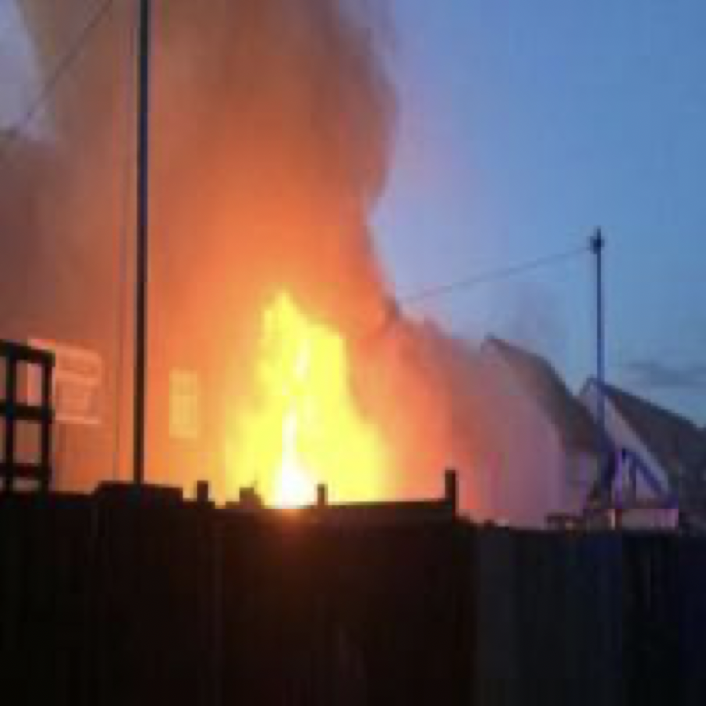
\includegraphics[width=4cm, height=4cm]{original} }}%
    \qquad
    \subfloat[\centering Brightened]{{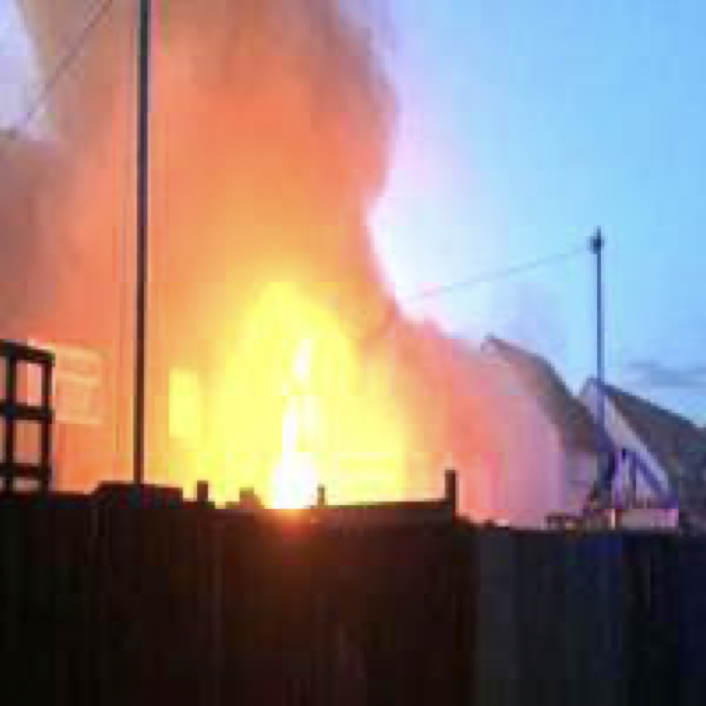
\includegraphics[width=4cm, height=4cm]{brightened} }}%
	\qquad
	\subfloat[\centering Noised]{{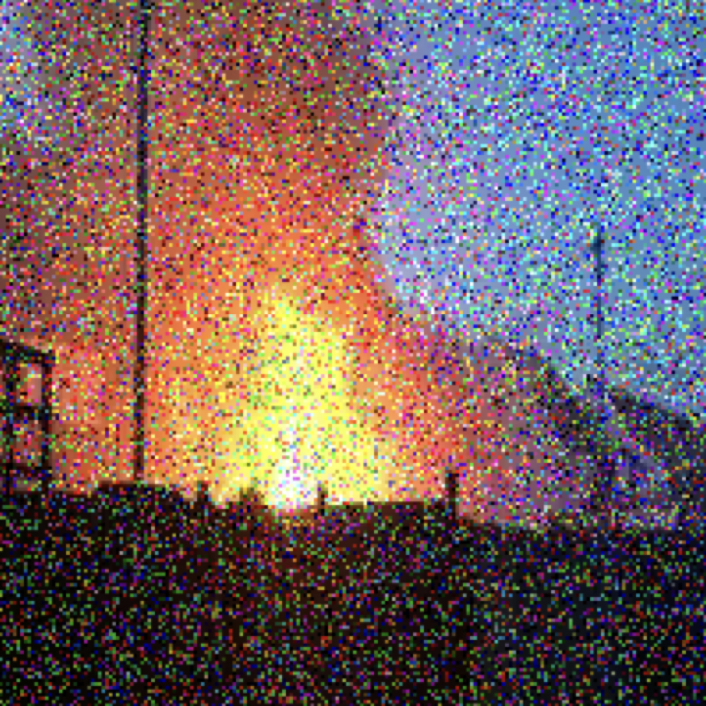
\includegraphics[width=4cm, height=4cm]{noised} }}%

	\subfloat[\centering Flipped]{{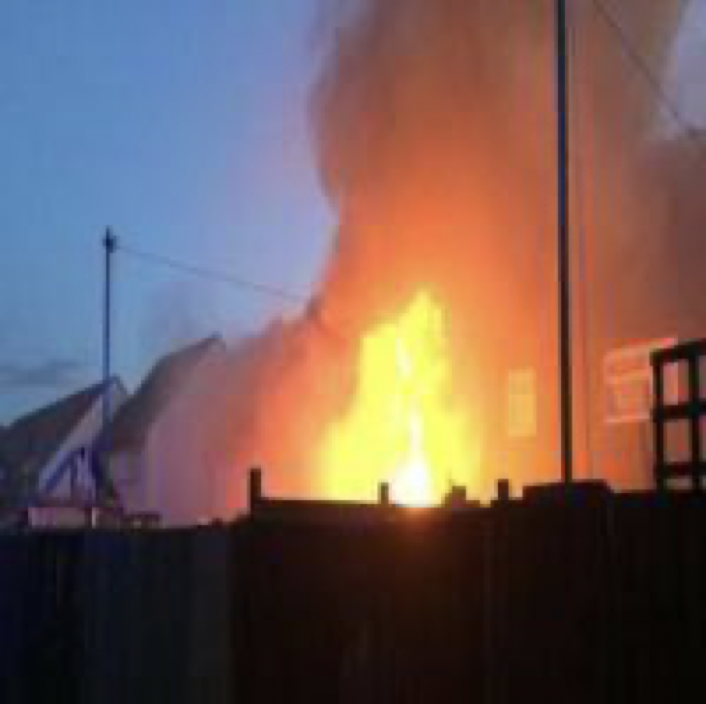
\includegraphics[width=4cm, height=4cm]{flipped} }}%
	\qquad
	\subfloat[\centering Jittered]{{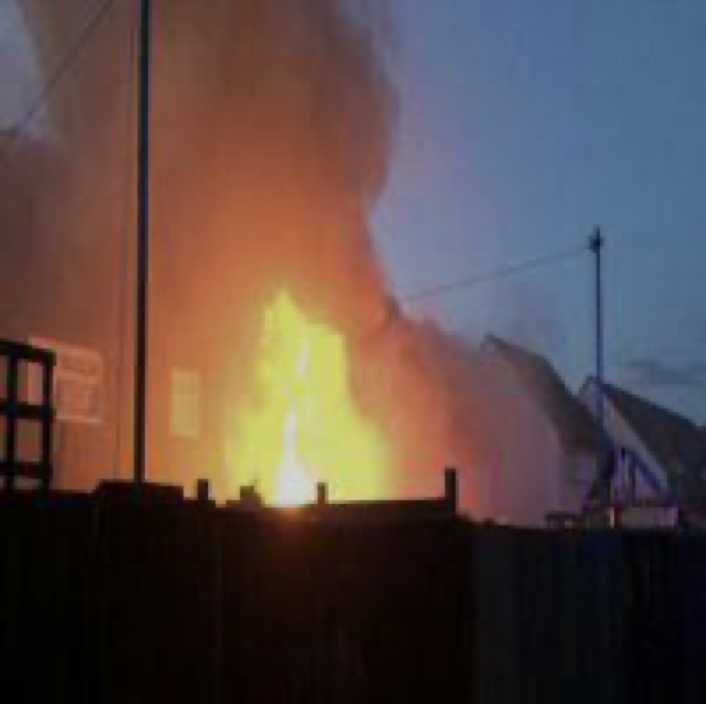
\includegraphics[width=4cm, height=4cm]{jittered} }}%
	\qquad
	\subfloat[\centering Zoomed]{{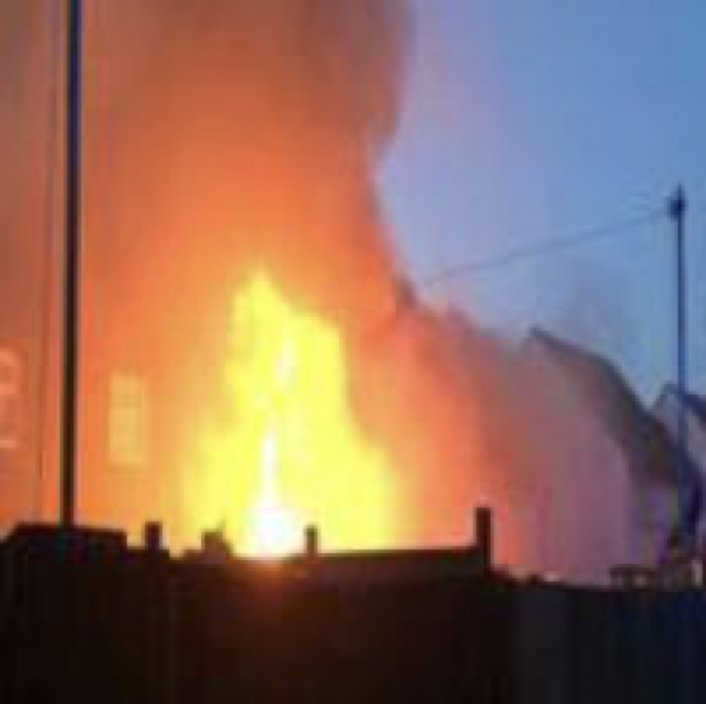
\includegraphics[width=4cm, height=4cm]{zoomed} }}%
    \caption{
		Example of augmented training data, using various methods
	}%
    \label{fig:example}%
\end{figure}

\section{Model and Methods}

80\%-20\% split in training and testing set and 85\%-15\% split in training and validation set
Hyperparameter tuning: 10 epochs, SGD optimizer, momentum=0.9, LR 0.001
We tried different neural networks among ResNet, MobileNet, and AlexNet to determine which model had the best performance.

\section{Results}

Graph goes here

ResNet best-performed with deeper layers and skip connections.
MobileNet performed worse than ResNet due to its streamlined architecture, which, while efficient, doesn’t capture complex patterns as effectively. AlexNet also performed worse than ResNet due to its relatively simpler architecture.


\section{Conclusions}

To combat potential overfitting, we may employ k-fold cross-validation to train the model on different subsets.
By applying semantic segmentation to our model, we can assign labels to pixels of the image to identify the precise region of a fire.
We can collect more edge case images with light sources to make the model more false-positive-proof.


\section{Citations, figures, tables, references}
\label{others}

These instructions apply to everyone, regardless of the formatter being used.

\subsection{Citations within the text}

Citations within the text should be based on the \texttt{natbib} package
and include the authors' last names and year (with the ``et~al.'' construct
for more than two authors). When the authors or the publication are
included in the sentence, the citation should not be in parenthesis using \verb|\citet{}| (as
in ``See \citet{Hinton06} for more information.''). Otherwise, the citation
should be in parenthesis using \verb|\citep{}| (as in ``Deep learning shows promise to make progress
towards AI~\citep{Bengio+chapter2007}.'').

The corresponding references are to be listed in alphabetical order of
authors, in the \textsc{References} section. As to the format of the
references themselves, any style is acceptable as long as it is used
consistently.

\subsection{Footnotes}

Indicate footnotes with a number\footnote{Sample of the first footnote} in the
text. Place the footnotes at the bottom of the page on which they appear.
Precede the footnote with a horizontal rule of 2~inches
(12~picas).\footnote{Sample of the second footnote}

\subsection{Figures}

All artwork must be neat, clean, and legible. Lines should be dark
enough for purposes of reproduction; art work should not be
hand-drawn. The figure number and caption always appear after the
figure. Place one line space before the figure caption, and one line
space after the figure. The figure caption is lower case (except for
first word and proper nouns); figures are numbered consecutively.

Make sure the figure caption does not get separated from the figure.
Leave sufficient space to avoid splitting the figure and figure caption.

You may use color figures.
However, it is best for the
figure captions and the paper body to make sense if the paper is printed
either in black/white or in color.
\begin{figure}[h]
	\begin{center}
		%\framebox[4.0in]{$\;$}
		\fbox{\rule[-.5cm]{0cm}{4cm} \rule[-.5cm]{4cm}{0cm}}
	\end{center}
	\caption{Sample figure caption.}
\end{figure}

\subsection{Tables}

All tables must be centered, neat, clean and legible. Do not use hand-drawn
tables. The table number and title always appear before the table. See
Table~\ref{sample-table}.

Place one line space before the table title, one line space after the table
title, and one line space after the table. The table title must be lower case
(except for first word and proper nouns); tables are numbered consecutively.

\begin{table}[t]
	\caption{Sample table title}
	\label{sample-table}
	\begin{center}
		\begin{tabular}{ll}
			\multicolumn{1}{c}{\bf PART} & \multicolumn{1}{c}{\bf DESCRIPTION}
			\\ \hline \\
			Dendrite                     & Input terminal                      \\
			Axon                         & Output terminal                     \\
			Soma                         & Cell body (contains cell nucleus)   \\
		\end{tabular}
	\end{center}
\end{table}

\subsubsection*{Author Contributions}
If you'd like to, you may include  a section for author contributions as is done
in many journals. This is optional and at the discretion of the authors.

\subsubsection*{Acknowledgments}
Use unnumbered third level headings for the acknowledgments. All
acknowledgments, including those to funding agencies, go at the end of the paper.

\bibliography{iclr2023_conference}
\bibliographystyle{iclr2023_conference}
